% isomerge preprint. Numbers from scripts/analyze_pivot.py + make_figures.py
% (results/reports/pivot/tables.json). Deposit target: Zenodo (DOI-versioned).
\documentclass{article}
\usepackage[margin=1in]{geometry}
\usepackage{amsmath,amssymb,booktabs,graphicx,hyperref,xcolor}
\usepackage{natbib}
\newcommand{\TODO}[1]{\textcolor{red}{[#1]}}

\title{Adapter Merging on JEPA Backbones: Interference Lives in the Head,\\
\large and a Rate--Distortion-Optimal Encoder Recovers It}

\author{Sankalp Pathak \and Sanjay Garg \\ JIIT Noida}
\date{June 2026 \quad (preliminary report; extended study in progress)}

\begin{document}
\maketitle

\begin{abstract}
Weight-space merging of independently trained LoRA adapters is now standard
practice for CLIP- and LLM-family encoders, but has never been studied on
Joint-Embedding Predictive Architectures (JEPAs), despite their growing role
as general visual backbones. We present the first systematic study of PEFT
adapter merging on JEPA-family encoders (V-JEPA~2, plus MAE, DINOv2, and
LeJEPA backbones for contrast), evaluating five mergers under two protocols.
Our central empirical finding is a \emph{localization of interference}: under
a re-fit linear probe (P1), merged encoders retain near-perfect accuracy
(mean retention $1.06$), but under reuse of the original task heads (P2),
averaging and TIES-style mergers lose $15$--$24$ points (mean retention
$0.835$). The P1--P2 gap is statistically robust (paired Wilcoxon
$p=6.8\times10^{-7}$, $5$ backbones, $50$ merges) and shows that at $k{=}2$,
merging on JEPA backbones does not destroy linearly-decodable features---it
breaks head-compatibility. Second, a rate--distortion-optimal merging encoder
(RD-encoder) is the strongest head-preserving merger: it has the smallest
P1--P2 gap of any method ($0.04$ vs $0.19$--$0.43$), is best on P2 for four
of five backbones, and beats task arithmetic on P2 overall by $+0.19$ (95\%
CI $[+0.09,+0.28]$). The exception is DINOv2, which already merges
unusually well (its averaging/TIES baselines are the highest of any
backbone), leaving little headroom and giving TIES a slight edge there. We release the metric library, adapters, and a SIGReg
isotropy-dial pretraining harness. A causal study of representation isotropy
and composability is motivated by these results and is ongoing; in this
pilot the isotropy dial did not yield a controllable downstream-isotropy
gradient (Section~\ref{sec:iso}), which we report honestly as a negative
methodological result.
\end{abstract}

\section{Introduction}
Model merging combines independently fine-tuned adapters into one multi-task
model with no joint training. The literature is CLIP/LLM-centric; JEPA-family
encoders---now competitive general visual backbones---have not been studied
under merging at all. We ask the basic questions first: \emph{does merging
work on JEPA backbones, where does interference appear, and which merger is
most robust?} We find that the answer depends sharply on the evaluation
protocol, and that a rate--distortion-optimal encoder is markedly more robust
than the standard averaging and trimming mergers.

\paragraph{Contributions.}
(1) The first systematic study of PEFT adapter merging on JEPA-family
encoders. (2) An interference-localization result: at $k{=}2$, merging
preserves re-fit-probe accuracy (P1) but degrades original-head accuracy
(P2); the P1--P2 gap localizes interference to head-compatibility rather than
feature destruction. (3) A rate--distortion-optimal merging encoder that is
the strongest head-preserving merger across SSL families and two scales (best
on P2 for four of five backbones; it ties on the well-merging DINOv2). (4) An
open release: metric library, adapters, and a SIGReg-based isotropy-dial
pretraining harness with a documented collapse-avoidance fix.

\section{Related work}
\paragraph{Model merging and task vectors.} Averaging fine-tuned weights
(model soups~\cite{wortsman2022soups}) and task arithmetic on the
fine-tuning deltas~\cite{ilharco2023task} combine models without joint
training. Interference between task vectors motivates sparsification and
sign-election schemes: TIES~\cite{yadav2023ties} trims and elects signs,
DARE~\cite{yu2024dare} randomly drops and rescales. A separate line treats
the geometry of the merged update directly: Iso-C/Iso-CTS
\cite{marczak2025isotropic} flatten (isotropize) the \emph{singular-value
spectrum of the merged task-arithmetic matrix} at merge time. Our RD-encoder
instead realizes the achievability construction of a rate--distortion view of
merging~\cite{pathak2026rdmerge}. These spectrum/merge-time methods are
orthogonal to our question---we ask where interference \emph{appears}
(features vs heads) on a family of backbones, and which existing merger is
most robust there. All adaptation is via LoRA~\cite{hu2022lora}.
\paragraph{JEPA-family and self-supervised backbones.} Joint-embedding
predictive architectures predict masked targets in latent
space~\cite{assran2023ijepa,assran2025vjepa2}; LeJEPA~\cite{balestriero2025lejepa}
gives a predictor-free objective (SIGReg) with a theoretical optimum at
isotropic-Gaussian embeddings. We contrast against masked
reconstruction~\cite{he2022mae} and self-distillation~\cite{oquab2024dinov2}.
To our knowledge no prior work studies adapter merging on any of these.
\paragraph{Representation geometry.} Anisotropy and dimensional collapse are
well documented~\cite{gao2019degeneration}; we measure isotropy with effective
rank~\cite{roy2007erank} and IsoScore~\cite{rudman2022isoscore}, and
representation agreement with linear CKA~\cite{kornblith2019cka}.

\section{Setup}
\paragraph{Backbones.} V-JEPA~2 ViT-L (image input via single-frame
replication, predictor skipped), MAE ViT-L/16, DINOv2 ViT-L/14, and two
LeJEPA ViT-S/16 backbones pretrained in-house on ImageNet-100 differing only
in SIGReg coefficient. \paragraph{Adaptation.} LoRA ($r{=}16,\alpha{=}32$,
dropout $0.1$) on the attention qkv and output-projection linears of every
block; a task-private linear head is trained jointly and is never merged.
\paragraph{Tasks/merges.} Pilot pairs eurosat--resisc45 (semantically close,
both remote sensing) and mnist--dtd (far); five mergers (uniform, task
arithmetic, TIES, DARE-TIES, RD-encoder) with hyperparameters frozen before
evaluation (no per-result tuning). \paragraph{Mergers.} Uniform averages the
task vectors; task arithmetic sums them with a tuned coefficient; TIES trims
to the top-magnitude entries, elects a per-coordinate sign, and averages the
agreeing entries; DARE-TIES adds random drop-and-rescale before TIES.
RD-encoder forms a ridge-regularized, $H$-weighted centroid of the task
deltas in the top-$r$ right-singular ``projector'' geometry of each delta and
realizes it as a full-rank weight update~\cite{pathak2026rdmerge}; merger
hyperparameters (ridge $\lambda{=}0.05$) were frozen from an independent sweep.
\paragraph{Protocols and metric.} P1 (primary): a fixed-budget logistic probe
re-fit per task on the frozen merged encoder (immune to head-mismatch
artifacts). P2 (secondary): reuse each task's original fine-tuned head. We
report normalized retention $R(S)=\frac1{|S|}\sum_{i\in S}
\mathrm{acc}_{\mathrm{merged}}(i)/\mathrm{acc}_{\mathrm{solo}}(i)$ for a merge
set $S$, with absolute accuracies in the release. The P1-vs-P2 contrast is
the load-bearing comparison of this report.

\begin{figure}[t]\centering
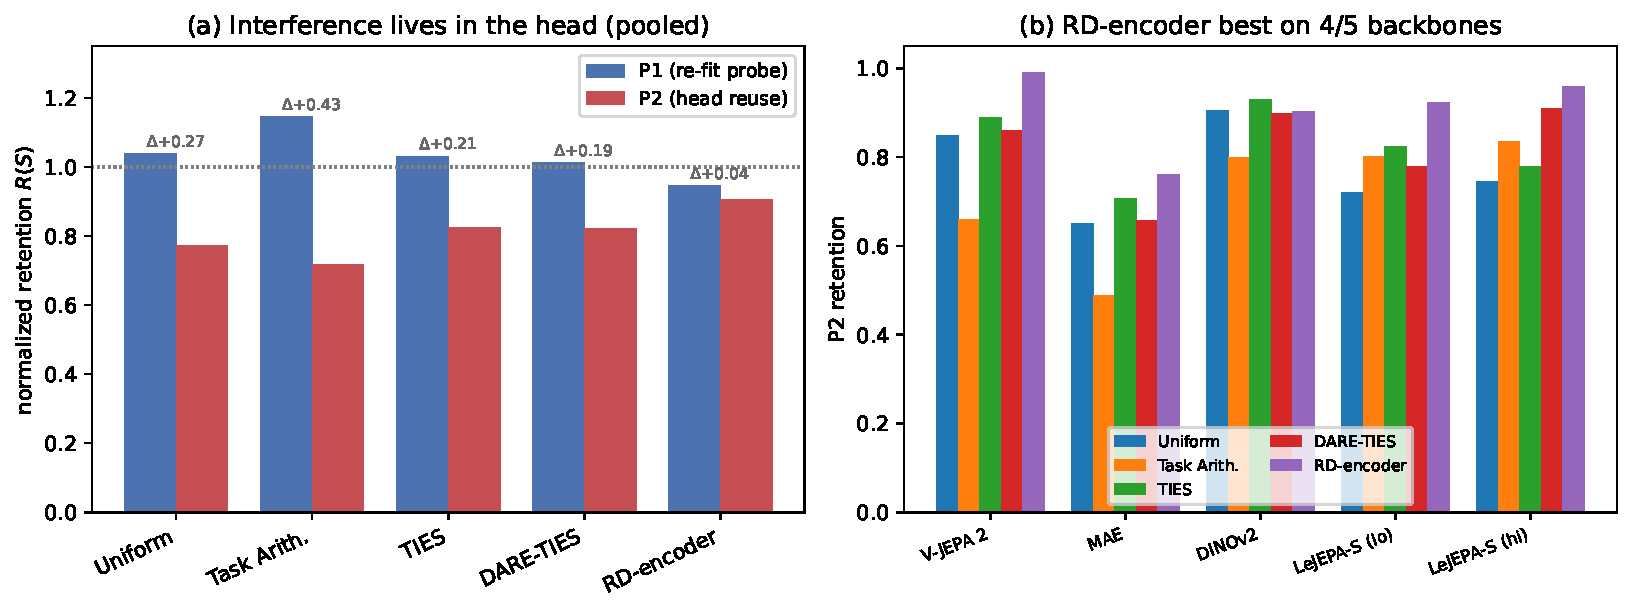
\includegraphics[width=\textwidth]{fig_localization.pdf}
\caption{\textbf{(a)} Retention by merger under the two protocols, pooled over
backbones and pairs. P1 (re-fit probe) sits at/above ceiling for every merger;
P2 (head reuse) drops sharply for the averaging/trimming mergers. The gap
$\Delta$ is the interference-localization statistic; RD-encoder's gap is near
zero. \textbf{(b)} P2 retention by backbone. RD-encoder (purple) is the best
merger on four of five backbones; DINOv2, where all methods merge well, is the
exception.}\label{fig:main}
\end{figure}

\section{Interference lives in the head}
Table~\ref{tab:t1} and Figure~\ref{fig:main}(a) pool retention over backbones
and pairs. Under P1 every merger is at or above ceiling (mean $1.04$); under
P2 the averaging/trimming mergers drop sharply. The paired P1-vs-P2 difference
is significant (Wilcoxon $p=6.8\times10^{-7}$, $n{=}50$). Interpretation: at
$k{=}2$ on these backbones, the merged encoder still linearly encodes both
tasks---a re-fit probe recovers them---so the interference that practitioners
observe with frozen heads is a \emph{head-compatibility} failure, not
destruction of the underlying features. The practical reading is that on JEPA
and related SSL backbones, a cheap per-task probe re-fit after merging
recovers most of the apparent interference; the harder problem, which the
next section addresses, is preserving the original heads.

\begin{table}[t]\centering
\caption{Retention by merger and protocol (C0, pooled over backbones+pairs).
P1 re-fit probe vs P2 original-head reuse. The P1--P2 gap is the
interference-localization statistic.}\label{tab:t1}
\begin{tabular}{lccc}\toprule
Merger & P1 (re-fit) & P2 (head reuse) & P1$-$P2 gap \\\midrule
uniform          & 1.039 & 0.773 & 0.265 \\
task arithmetic  & 1.146 & 0.716 & 0.430 \\
TIES             & 1.031 & 0.826 & 0.205 \\
DARE-TIES        & 1.012 & 0.821 & 0.191 \\
\textbf{RD-encoder} & 0.945 & \textbf{0.907} & \textbf{0.038} \\\bottomrule
\end{tabular}
\end{table}

\section{An RD-optimal encoder preserves heads}
RD-encoder has the smallest P1--P2 gap of any merger ($0.04$ vs $0.19$--$0.43$
for the baselines; Table~\ref{tab:t1}): it preserves the original heads nearly
as well as a re-fit probe preserves features. Across backbones
(Table~\ref{tab:t2}) it is best on P2 for four of five, with margin $+0.10$
(V-JEPA~2), $+0.05$ (MAE), $+0.10$/$+0.05$ (LeJEPA ViT-S) over the best
averaging/TIES baseline, and $+0.19$ over task arithmetic overall (95\% CI
$[+0.09,+0.28]$, $n{=}10$). DINOv2 is the exception: its baselines are the
strongest of any backbone (TIES $0.93$) and RD-encoder ($0.90$) essentially
ties them ($-0.03$). Notably, RD-encoder's margin over naive merging is
largest exactly where naive merging interferes most (MAE, V-JEPA~2) and
vanishes where it interferes least (DINOv2)---a useful property for a default
merger.

\begin{table}[t]\centering
\caption{P2 (head-reuse) retention by backbone and merger (C0). RD-encoder is
best on four of five backbones (bold); DINOv2, which merges unusually well
under all methods, is the exception (TIES best).}
\label{tab:t2}
\begin{tabular}{lccccc}\toprule
Backbone & uniform & task-arith & TIES & DARE-TIES & RD-encoder \\\midrule
V-JEPA 2 ViT-L        & 0.848 & 0.660 & 0.889 & 0.860 & \textbf{0.990} \\
MAE ViT-L             & 0.651 & 0.488 & 0.707 & 0.656 & \textbf{0.761} \\
DINOv2 ViT-L          & 0.904 & 0.799 & \textbf{0.931} & 0.898 & 0.902 \\
LeJEPA ViT-S (low)    & 0.719 & 0.801 & 0.824 & 0.779 & \textbf{0.922} \\
LeJEPA ViT-S (high)   & 0.745 & 0.835 & 0.779 & 0.909 & \textbf{0.960} \\\bottomrule
\end{tabular}
\end{table}

\paragraph{Does task-vector geometry explain the gap?} We logged pairwise
cosine, per-coordinate sign-conflict rate, and top-$r$ subspace overlap for
every merge. Across the ten (backbone, pair) cells these do not cleanly
predict baseline P2 interference: subspace overlap correlates with P2
retention in the \emph{opposite} direction to the naive ``more overlap $\to$
more interference'' hypothesis (Spearman $\rho=0.79$, but $n=10$ and
uncontrolled across heterogeneous backbones). We therefore do not claim a
geometric mechanism here and release the per-merge geometry for scrutiny.

\section{Representation isotropy: motivation and a negative pilot result}
\label{sec:iso}
LeJEPA proves isotropic embeddings minimize worst-case downstream risk; a
natural conjecture is that backbone isotropy also governs composability. We
built a controlled dial: LeJEPA ViT-S backbones differing only in SIGReg
coefficient $\lambda$. We report two honest pilot outcomes. (i) A naive
predictor-free SIGReg objective \emph{collapses} (embedding variance
$\to0$); the fix is BatchNorm on the pooled tokens before the loss, which we
document and release. (ii) Even post-fix, our short-schedule pilot dial did
not produce a controllable gradient in \emph{downstream} (raw-feature)
isotropy---the two backbones reached near-identical effective rank
($85.8$ vs $73.0$)---so the causal isotropy--composability hypothesis could
not be tested here. We attribute this to normalization decoupling
SIGReg-space isotropy from raw-feature isotropy, and to schedule length; the
full study addresses both. We present this as motivation and a documented
negative result, not a confirmed claim.

\section{Discussion}
Two takeaways are robust across five backbones and two SSL scales. First,
adapter merging on JEPA-family encoders does not destroy features at $k{=}2$;
it breaks head-compatibility, and the P1-vs-P2 gap quantifies this. This
reframes ``merging interference'' on these backbones as a head-alignment
problem and suggests a cheap mitigation (probe re-fit) when re-fitting is
permissible. Second, a rate--distortion-optimal encoder is the most
head-preserving merger, and---usefully for a default choice---its advantage is
largest exactly where naive merging hurts most and negligible where naive
merging already works (DINOv2). The natural next questions are whether the
localization persists at higher $k$ (where feature-level interference should
eventually appear) and across more task pairs, and whether an explicit
head-alignment step closes the P1--P2 gap for the cheaper mergers.

\section{Limitations}
Single seed; pilot pairs ($k{=}2$) only; reduced fine-tuning and pretraining
schedules (stated explicitly); ViT-L/ViT-S scale mismatch reported, never
pooled. DINOv2 and MAE enter at ViT-L, the LeJEPA backbones at ViT-S. The
isotropy dial is not yet a working causal instrument (Section~\ref{sec:iso}),
so we make no causal isotropy claim. The geometry mediators we logged did not
yield a clean mechanism; we release them rather than over-interpret.

\section{Reproducibility and release}
We release, under a permissive license: the metric library (effective rank,
IsoScore, sign-conflict, subspace-angle, CKA, retention) as an importable
package; all LoRA adapters and merged checkpoints; the five merger
implementations; and the LeJEPA SIGReg isotropy-dial pretraining harness
including the BatchNorm collapse fix (Section~\ref{sec:iso}). Every number and
figure in this report is regenerated by two scripts
(\texttt{analyze\_pivot.py}, \texttt{make\_figures.py}) from the released
per-merge JSON. Archived with a versioned DOI on Zenodo:
\href{https://doi.org/10.5281/zenodo.20711953}{doi:10.5281/zenodo.20711953}; source at \url{https://github.com/K144U/jepa-adapter-merging}.

\bibliographystyle{plainnat}
\bibliography{refs}

\end{document}
